\section{円筒シェルの座屈}
この例では、軸方向に圧縮された円筒形シェルの線形座屈解析を行います。その寸法は:
\begin{itemize}
\item 直径: 300 mm
\item 長さ:600mm
\end{itemize}
ジオメトリーは、CADソフトウェアでサーフェスとしてモデリングされています。
\begin{enumerate}
\item
  {[}mm, ton, s, °C{]}単位の新規ファイルを作成し、ステップ形式のジオメトリをPrePoMaxにインポートします。
  次に、パーツをメッシュ分割します。
  ここでは、最大要素サイズとして10mmを選択し、四分割メッシュを有効にして、その他の設定は変更しませんでした(図\ref{fig:09-01})。
	\begin{figure}[H]
	\centering
	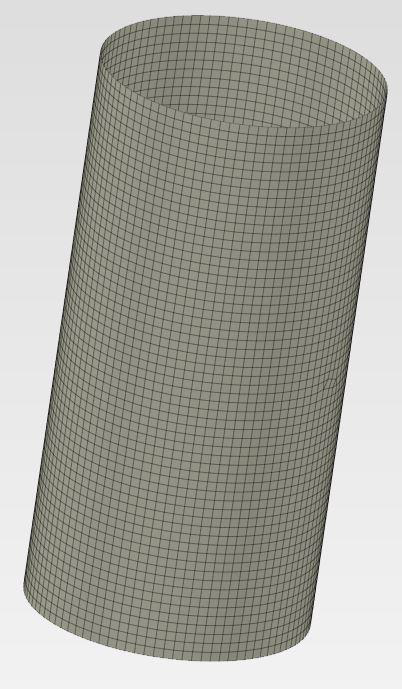
\includegraphics[width=53mm]{fig/09-01.png}
	\caption{円筒シェル - メッシュ}
	\label{fig:09-01}
	\end{figure}
	\vspace{-\baselineskip}
\item
  新しい材料を定義し、弾性挙動を加え、ヤング率を210000MPa、ポアソン比を0.3と指定します。
  先に作成した材料を参照して新しいシェルセクションを作成し、そのセクションがこのパーツに割り当てられるように円筒シェルを選択します。
  厚さを5mmに指定します。
\item
  座標(0, 0, 600)に基準点を作成します。
  この基準点とシェルのエッジを使って剛体拘束を定義します。
\item
  新しい座屈ステップを追加し、座屈係数の数を5に設定します。
  シェルの下部エッジに割り当てられた固定境界条件を作成します。
  集中荷重を定義し、シェルの上端に接続された基準点に適用します。
  この荷重には-1Nを指定します(図\ref{fig:09-02})。
	\begin{figure}[H]
	\centering
	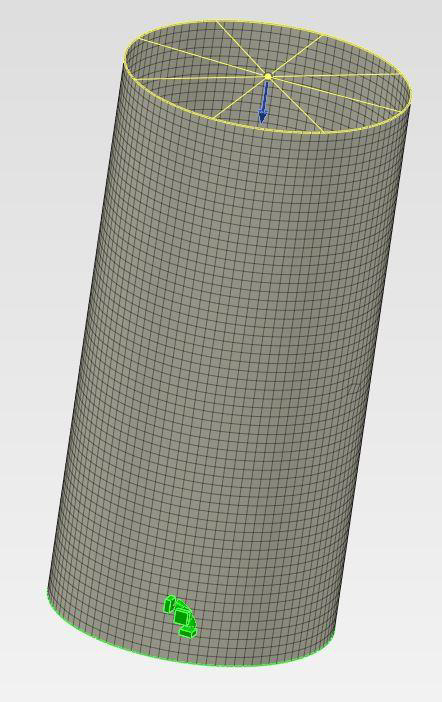
\includegraphics[width=56mm]{fig/09-02.png}
	\caption{円筒シェル - 境界条件と荷重}
	\label{fig:09-02}
	\end{figure}
	\vspace{-\baselineskip}
\item
  解析を実行し、解析が終了したら結果を開きます。
  変形のスケール係数を10000に設定し、座屈モードの形状を確認します。
  そのうちの1つ(\#4)を下の画像に示します(図\ref{fig:09-03})。
  分析的に計算された限界荷重は1.9964-107ですが、シミュレーションでは1.9024-107となります。
	\begin{figure}[H]
	\centering
	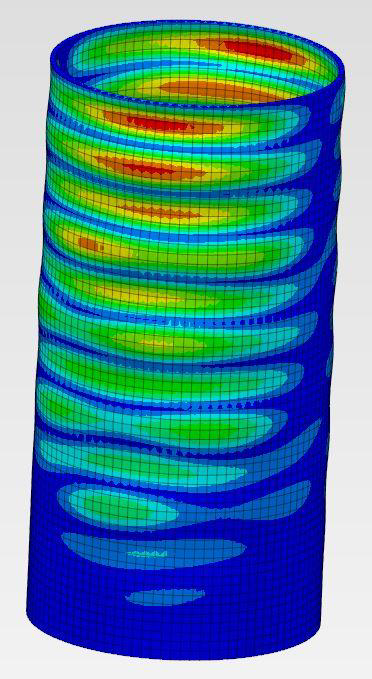
\includegraphics[width=56mm]{fig/09-03.png}
	\caption{円筒シェル - 座屈モード形状 \#4}
	\label{fig:09-03}
	\end{figure}
	\vspace{-\baselineskip}
\end{enumerate}